\documentclass{article}
%%%%%%%%%%%%%%%%%%%%%%%%%%%%%%%%%%%%%%%%%%%%%%%%%%%%%%%%%%%%%%%%%%%%%%%%%%%%%%%%%%%%%%%%%%
\title{Ensayo de costos - Visita a Xamán}
\date{2020-Mar-02}
\author{David Gabriel Corzo Mcmath}
%%%%%%%%%%%%%%%%%%%%%%%%%%%%%%%%%%%%%%%%%%%%%%%%%%%%%%%%%%%%%%%%%%%%%%%%%%%%%%%%%%%%%%%%%%
\usepackage{davidcorzo}
\usepackage[top=0.5in,bottom=0.5in, left=1in, right=1in]{geometry}
\packagesneeded
%%%%%%%%%%%%%%%%%%%%%%%%%%%%%%%%%%%%%%%%%%%%%%%%%%%%%%%%%%%%%%%%%%%%%%%%%%%%%%%%%%%%%%%%%%

\begin{document}
\maketitle
\tikzblockdefinitions

\section{Visita a la empresa Xamán}
Xamán es una empresa que se dedica a la producción de cerveza artesanal, entre las cosas interesantes que se pudo absorber de la visita a dicha empresa fue el proceso de la cerveza y las distintas formas de elaborarla. 


%%%%%%%%%%%%%%%%%%%%%%%%%%%%%%%%%%%%%%%%%%%%%%%%%%%%%%%%%%%%%%%%%%%%%%%%%%%%%%%%%%%%%%%%%%
\section{Costos y análisis económico}
El tour de la planta de producción fue dada por uno de los fundadores de la empresa, él en su presentación comentaba al grupo acerca de las altas barreras de entrada al negocio. Dado a la necesidad de licencias sanitarias y el tiempo que se toma en aprobarlas es tardado el proceso de entrar al negocio, en el caso de Xamán se tardó un tiempo récord de un poco más de un año.

\begin{center}
   \begin{longtable}{ | p{4.5cm} | p{12cm} | }
       \hline
            \textbf{Costos Variables: }  & 
            \begin{itemize}
                \item Cuarto frío, energía eléctrica.
                \item Materia prima: malta, lúpulo, agua.
                \item Gastos de venta como publicidad, objetos con su marca.
                \item Botellas y las etiquetas de las botellas.
                \item Gastos de distribución.
                \item Costos de limpieza que se incurren al terminar cada lote.
            \end{itemize} \\ 

       \hline
            \textbf{Costos fijos: } & 
            \begin{itemize}
                \item Costos de gerente de producción y dos operarios.
                \item Mantenimiento del boiler o caldera cada mes.
                \item Mantenimiento del brewer una vez al año.
                \item El costo fijo del salario de dos operarios.
                \item Dividendos mensuales entre los fundadores, se intenta pagar a los fundadores remuneración proporcional a un precio de mercado.
                \item Costos de alquiler y de arrendamiento.
                \item Renta de local.
                \item Gastos administrativos.
                \item Gastos de distribución.
            \end{itemize} \\ 
            
        \hline
            \textbf{Costos Marginales: } & 
            \begin{itemize}
                \item Se produce por lotes para disminuir el costo, el costo total se disminuye cuando se produce al por mayor.
                \item El costo total llega a un punto óptimo antes de empezar a subir, este punto óptimo es el que se intenta llegar, en este caso producir las unidades que se venderán y que minimice el costo es el objetivo. Un ejemplo aparte del de producción por lotes es la adquisición de las botellas y de las etiquetas al por mayor, al adquirir estos bienes al por mayor se puede acordar con los proveedores un precio más bajo, marginalmente se observa que conviene adquirir al por mayor en este caso.
            \end{itemize} \\ 
            
        \hline
            \textbf{Costos irrecuperables: } & 
            \begin{itemize}
                \item Costos de emisión de licencias.
                \item Costos de permisos sanitarios.
                \item Costos de remodelación y el piso.
            \end{itemize} \\ 
        \hline
            \textbf{Rendimientos de escala: } & 
            \begin{itemize}
                \item Si se fuesen a duplicar todos los factores de producción se verían rendimientos de desescala debido a que la operación está limitada en un punto solamente que es el cuello de botella que hay en el tanque de fermentación.
            \end{itemize} \\ 
        \hline
            \textbf{Economías de escala: } & 
            \begin{itemize}
                \item Si se fuese a comprar otro tanque de fermentación afirmó el empresario, se pudiera procesar por lo menos el doble de lo que se produce, esto no sería duplicar el costo, sería un ejemplo de economía de escala.
            \end{itemize} \\ 
        \hline
            \textbf{Economías de alcance: } & 
            \begin{itemize}
                \item El empresario afirmaba que intentaban tercerizar partes que no fueran cerveza, si ellos producirán la botella, etiqueta y tapones de botella serían ineficientes, ellos sólo hacen la cerveza. 
            \end{itemize} \\ 
        \hline
            \textbf{Factores de producción (trabajo y capital): } & 
            \begin{itemize}
                \item Máquinas del proceso: brewer, boiler, molino, tanque de fermentación.
                \item Trabajadores: 2 operarios y un gerente de producción.
            \end{itemize} \\ 
        \hline
            \textbf{Precio del trabajo y precio del capital: } & 
            \begin{itemize}
                \item El precio del capital es su tasa de uso, es decir todo el monto depreciable de las máquinas en questión, un ejemplo sería la depreciación de la caldera o boiler ya que ese monto y el los intereses no ganados es lo que vale.
                \item El precio del trabajo es el salario de los trabajadores, en este caso el sueldo de los dos operarios y el gerente de producción serán parte del precio del trabajo.
            \end{itemize} \\ 
        \hline
            \textbf{Tiempo: } & 
            \begin{itemize}
                \item Son costos en su mayoría del corto plazo, esto por que tienen que ser incurridos en un lapso de tiempo menores o aproximadamente de un año. 
                \item A largo plazo todo es un costo variable.
            \end{itemize}  \\ 
        \hline
        
   \end{longtable}
\end{center}



%%%%%%%%%%%%%%%%%%%%%%%%%%%%%%%%%%%%%%%%%%%%%%%%%%%%%%%%%%%%%%%%%%%%%%%%%%%%%%%%%%%%%%%%%%
\section{Fotos}
% \begin{figure}[htbp]
\noindent
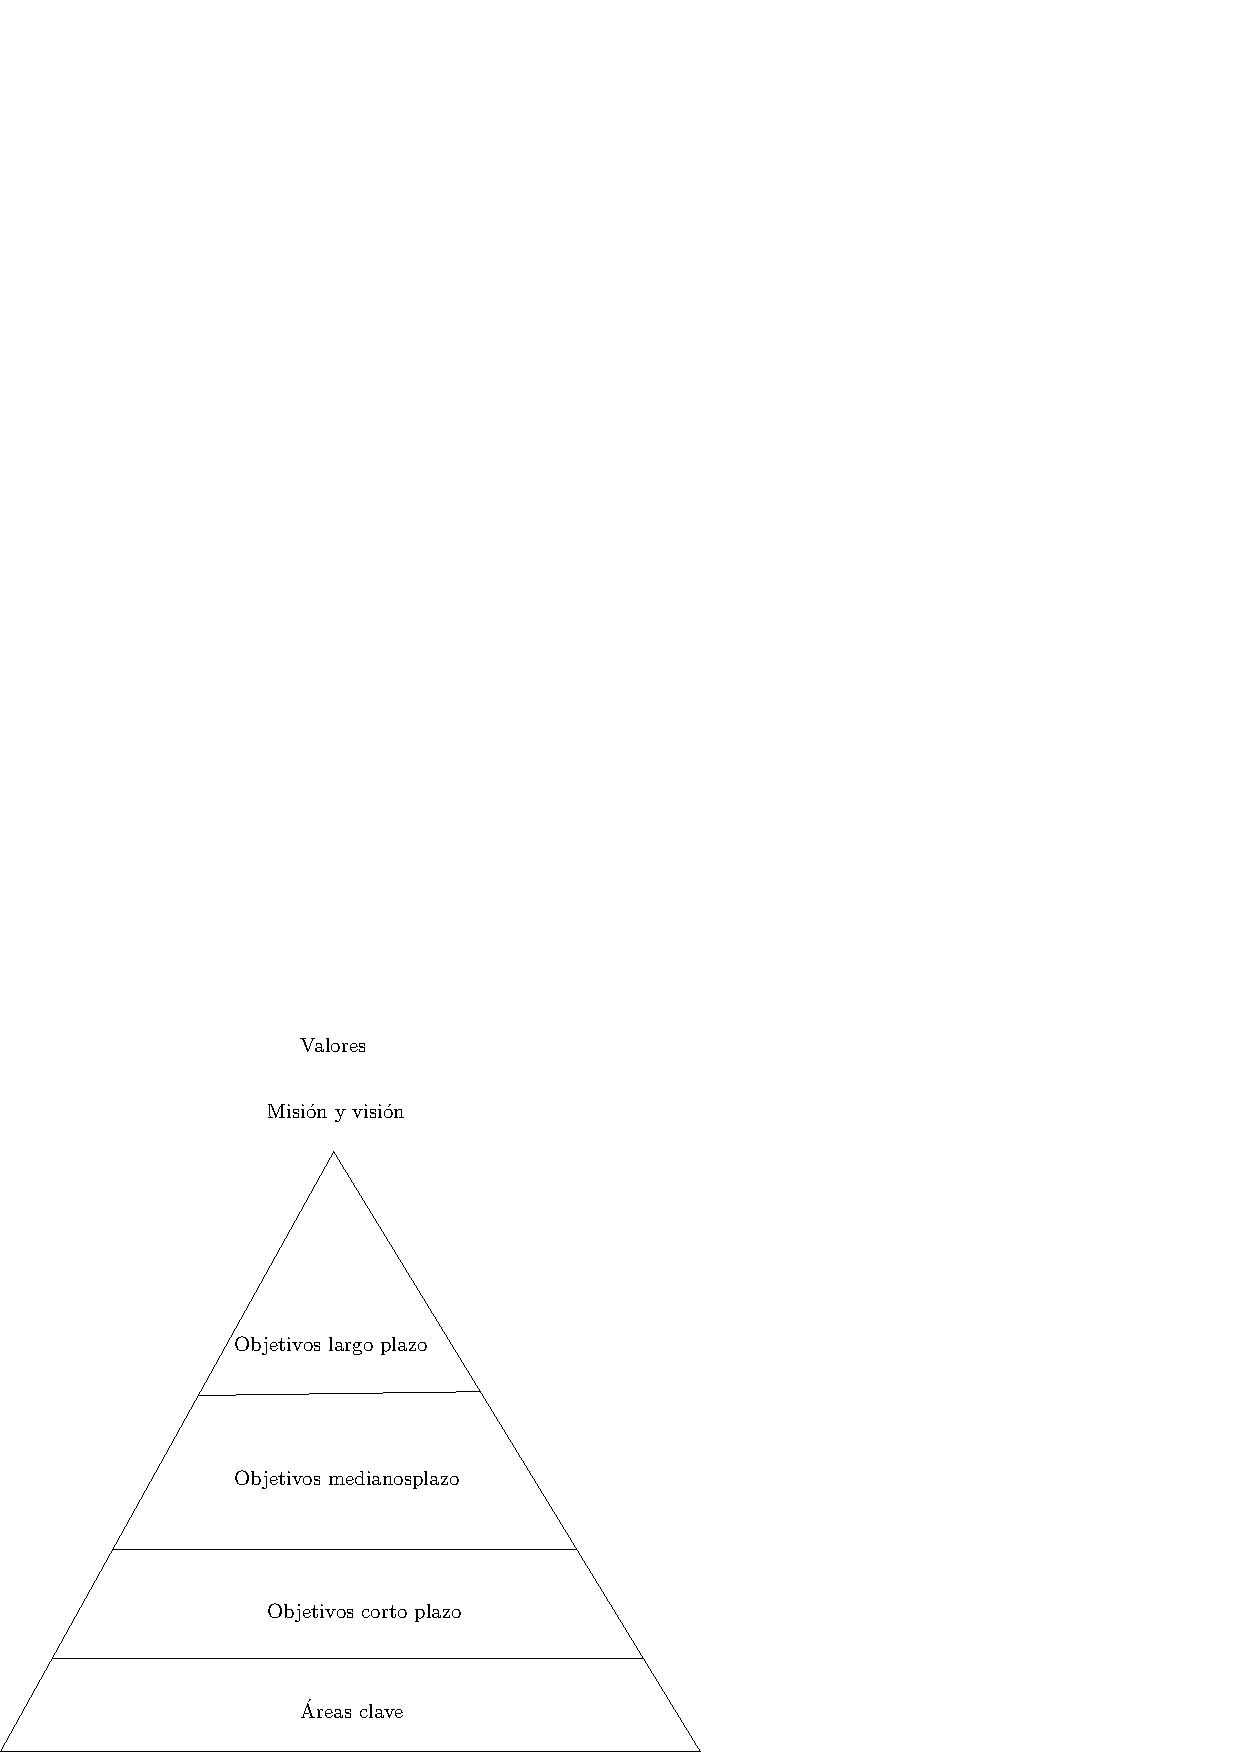
\includegraphics[width=6cm]{./img/01.JPG}
\includegraphics[width=6cm]{./img/02.JPG}
\includegraphics[width=6cm]{./img/03.JPG}
\includegraphics[width=6cm]{./img/04.JPG}
\includegraphics[width=6cm]{./img/05.JPG}
\includegraphics[width=6cm]{./img/06.JPG}
\includegraphics[width=6cm]{./img/07.JPG}
\includegraphics[width=6cm]{./img/08.JPG}
% \includegraphics[width=6cm]{./img/09.JPG}
\includegraphics[width=6cm]{./img/10.JPG}
% \end{figure}



%%%%%%%%%%%%%%%%%%%%%%%%%%%%%%%%%%%%%%%%%%%%%%%%%%%%%%%%%%%%%%%%%%%%%%%%%%%%%%%%%%%%%%%%%%
\section{Extra: Proceso de elaboración de la cerveza}
\begin{center}    
    \begin{tikzpicture}[node distance = 4cm, auto]
        \node [block] (1) {1. Filtro de agua}; 
        \node [block,right of=1] (2) {2. Molino }; 
        \node [block,right of=2] (3) {3. El tanque de maseración}; 
        \node [block,right of=3] (4) {4. Boiling tank}; 
        \node [block,below of=4, node distance = 2cm,auto] (5) {5. Tanque de fermentación}; 
        \node [block,left of=5] (6) {6. Filtrado}; 
        \node [block,left of=6] (7) {7. Carbonatación}; 
        \node [block,left of=7] (8) {8. Empaquetado}; 

        \path [line] (1) -- (2);
        \path [line] (2) -- (3);
        \path [line] (3) -- (4);
        \path [line] (4) -- (5);
        \path [line] (5) -- (6);
        \path [line] (6) -- (7);
        \path [line] (7) -- (8);

    \end{tikzpicture}
\end{center}




\end{document}


